\documentclass{../../slides-style}

\slidetitle{Практика 1: Введение}{20.02.2025}

\begin{document}

    \begin{frame}[plain]
        \titlepage
    \end{frame}

    \section{Введение}

    \begin{frame}
        \frametitle{Что мы будем делать на практике}
        \begin{itemize}
            \item Опробовать знания, полученные из теоретического курса
            \item Не будем писать код
            \begin{itemize}
                \item Курс очень гуманитарный, но увы, это тоже надо уметь
            \end{itemize}
            \item Будем \enquote{разрабатывать} воображаемые проекты
            \begin{itemize}
                \item Для этого их придётся придумать
                \item Можно взять проект с ЧМВ, можно --- учебную практику
            \end{itemize}
            \item Часть заданий будет прямо на паре, часть --- дома
            \begin{itemize}
                \item Будут командные задачи с дедлайном в неделю, выдаваемые после лекций
                \item На практике --- разбираем решения
            \end{itemize}
        \end{itemize}
    \end{frame}

    \begin{frame}
        \frametitle{Рекомендованная литература}
        \begin{footnotesize}
            \begin{itemize}
                \item \textbf{Роберт Гласс} Программирование и конфликты
                \item \textbf{Т. Питерс} Основы. Лидерство.
                \item \textbf{П.Ф. Друкер} Практика менеджмента
                \item Project Management Body of Knowledge
                \item \textbf{Т. ДеМарко, Т. Листер} Вальсируя с медведями: управление рисками в проектах по разработке программного обеспечения.
                \item \textbf{Т. ДеМарко, Т. Листер} Балдеющие от адреналина и зомбированные шаблонами. Паттерны поведения проектных команд.
                \item \textbf{Т. ДеМарко, Т. Листер} Человеческий фактор. Успешные проекты и команды.
                \item \textbf{Т. ДеМарко} Deadline. Роман об управлении проектами.
                \item \textbf{Ф. Брукс} Мифический человеко-месяц
                \item \textbf{Дж. Рейнвотер} Как пасти котов
                \item \textbf{Э. Хант} Программист-прагматик. Путь от подмастерья к мастеру
                \item \textbf{Дж. Спольски} Джоэл о программировании
                \item \textbf{И. Соммервилл} Инженерия программного обеспечения
                \item ...
            \end{itemize}
        \end{footnotesize}
    \end{frame}

    \begin{frame}
        \frametitle{Что будет в курсе}
        \begin{footnotesize}
            \begin{itemize}
                \item Работа с требованиями
                \item Практики Agile-методологий (парное программирование, backlog, спринты)
                \item Декомпозиция и оценка
                \item Планирование и слежение за ходом проекта
                \item Тестирование, отслеживание ошибок
                \item Финансовый план
            \end{itemize}
        \end{footnotesize}
    \end{frame}

    \section{Пример проекта}

    \begin{frame}
        \frametitle{Пример проекта}
        Информационный портал студотдела
        \begin{itemize}
            \item Цель проекта:
            \begin{itemize}
                \item автоматизировать выдачу справок об обучении, приём заявлений на повышенную стипендию
            \end{itemize}
            \item Требования:
            \begin{itemize}
                \item облегчать процесс получения справки
                \item облегчать процесс подачи студентами заявлений
                \item снижать нагрузку на работников деканата
                \item клиентская часть должна корректно работать в Google Chrome, Mozilla Firefox, Opera
                \item система должна иметь возможность одновременно работать с не менее 100 запросов без существенных потерь производительности
                \item время обработки одного запроса должно быть не более 5 сек
            \end{itemize}
        \end{itemize}
    \end{frame}

    \begin{frame}
        \frametitle{Диаграмма случаев использования}
        \begin{center}
            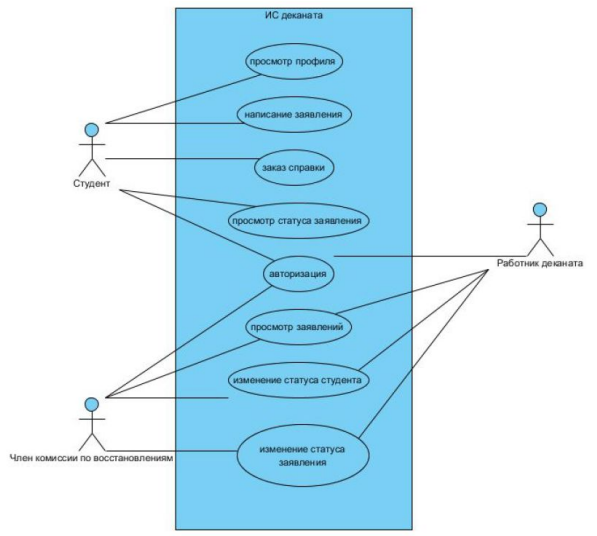
\includegraphics[width=0.6\textwidth]{useCase.png}
        \end{center}
    \end{frame}

    \begin{frame}
        \frametitle{Дерево задач}
        \begin{center}
            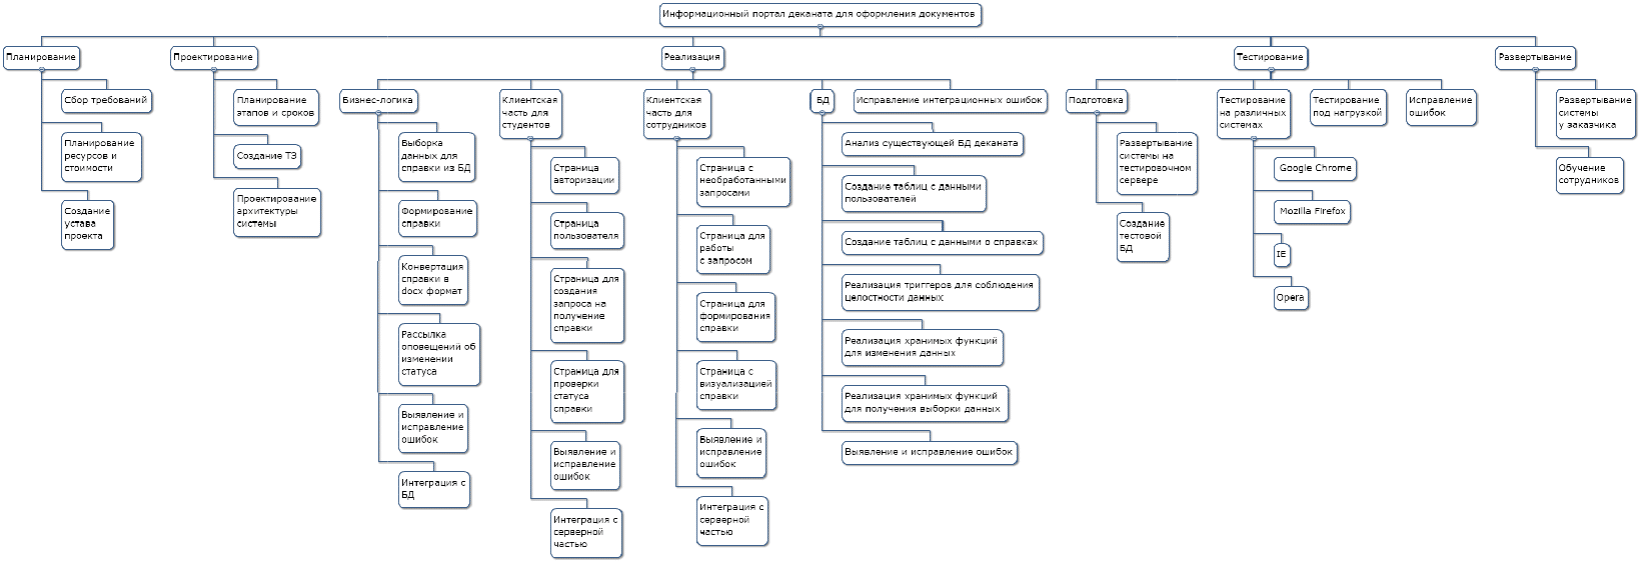
\includegraphics[width=\textwidth]{wbs.png}
        \end{center}
    \end{frame}

    \begin{frame}
        \frametitle{Риски}
        \begin{itemize}
            \item Недостатки планирования
            \begin{itemize}
                \item \textbf{Последствия} --- потеря времени, денег, в случае, если проект будет задержан на очень большое время --- потеря репутации
                \item \textbf{Вероятность} --- высокая
                \item \textbf{Угроза} --- высокая
                \item \textbf{Меры предотвращения} --- заложить дополнительно 80\% к времени и ресурсам, пригласить опытного специалиста для оценки проекта
            \end{itemize}
            \item Текучка кадров
            \begin{itemize}
                \item \textbf{Последствия} --- увеличение требуемого времени
                \item \textbf{Вероятность} --- высокая
                \item \textbf{Угроза} --- высокая
                \item \textbf{Меры предотвращения} --- попытаться найти средства для финансирования проекта, предложить участникам темы курсовых/дипломных работ в проекте
            \end{itemize}
            \item ...
        \end{itemize}
    \end{frame}

    \begin{frame}
        \frametitle{План проекта}
        \begin{center}
            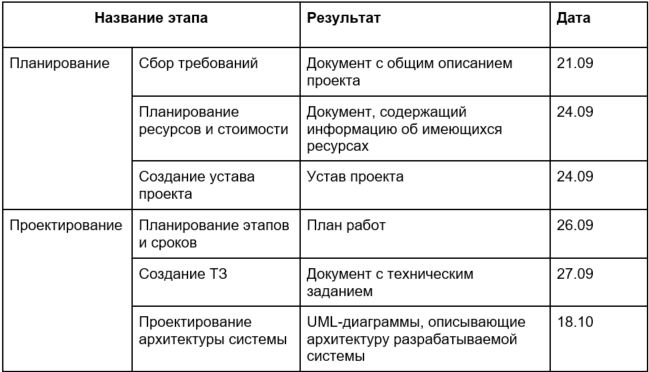
\includegraphics[width=0.8\textwidth]{plan1.png}
        \end{center}
    \end{frame}

    \begin{frame}
        \frametitle{План проекта (2)}
        \begin{center}
            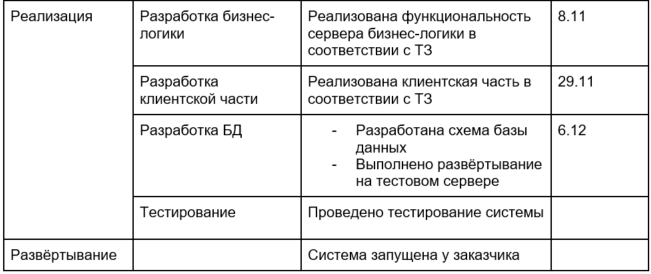
\includegraphics[width=0.8\textwidth]{plan2.png}
        \end{center}
    \end{frame}

    \begin{frame}
        \frametitle{Диаграмма Гантта}
        \begin{center}
            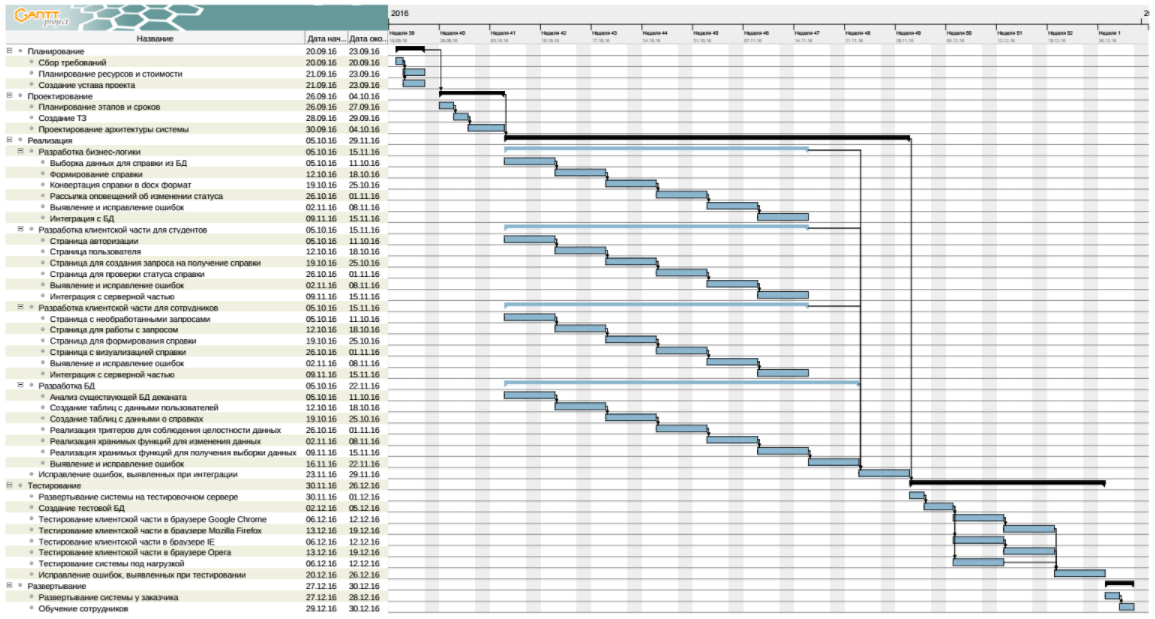
\includegraphics[width=\textwidth]{ganttChart.png}
        \end{center}
    \end{frame}

    \begin{frame}
        \frametitle{Описание вакансии}
        \begin{scriptsize}
            Молодая и успешная команда ищет разработчика C\# для создания и оптимизации кода серверной части информационной системы студотдела.

            Мы разрабатываем современный программный продукт, который поможет облегчить взаимодействие студентов и студотдела СПбГУ.

            Требования к кандидату:
            \begin{itemize}
                \item глубокое знание возможностей языка С\# и платформы .NET;
                \item понимание принципов разработки на ASP.NET;
                \item ...
            \end{itemize}

            Преимуществом будет:
            \begin{itemize}
                \item опыт работы с AngularJS, HTML5, CSS3, JavaScript, jQuery;
                \item ...
            \end{itemize}

            Обязанности:
            \begin{itemize}
                \item разработка сложной бизнес-логики;
                \item ...
            \end{itemize}

            Условия:
            \begin{itemize}
                \item использование в работе передовых технологий;
                \item возможность забить и не работать вообще.
            \end{itemize}
        \end{scriptsize}
    \end{frame}

    \begin{frame}
        \frametitle{План собеседования}
        \begin{small}
            \begin{itemize}
                \item Поздороваться
                \item Сказать, что экзаменатора пока нет, и что мне сказали сюда прийти встретить его и я просто его возможный будущий коллега
                \item \textbf{Коммуникабельность, поведенческие качества} --- завести дежурный разговор: спросить из какого он вуза, кафедры, если из СПбГУ, то спросить, кого он выбрал в научные руководители
                \item Далее получить сообщение (от себя же), что интервьюер не придёт, и что мне нужно самому провести собеседование
                \item \textbf{Технические навыки}
                \begin{itemize}
                    \item ​Когда вызываются статические конструкторы классов в C\#?
                    \item Каким образом можно перехватить добавление и удаление делегата из события?
                    \item Попросить объяснить принцип работы git
                \end{itemize}
                \item \textbf{Прошлый опыт} --- спросить, в каких проектах он до этого участвовал, в чём заключалась его конкретная задача
                \item ...
            \end{itemize}
        \end{small}
    \end{frame}

    \section{Домашнее задание}

    \begin{frame}
        \frametitle{Домашнее задание}
        \begin{itemize}
            \item Разделиться на команды по 3 человека
            \item Придумать проект, для которого будете писать документацию
            \begin{itemize}
                \item Это может быть ваша нынешняя или прошлая учебная практика, проект для курса ЧМВ или вообще выдуманный с нуля проект
                \item Он должен быть достаточно содержателен, хотя бы на пару человеколет работы
                \item Реализовывать его в ходе курса будет не нужно
                \item Хорошие выдуманные проекты можно будет в следующем году представить как осеннюю практику второго курса или вынести на ЛШ
            \end{itemize}
            \item Подготовить презентацию на 10 минут с представлением идеи проекта
            \item Дедлайн --- \textbf{6 марта}
        \end{itemize}
    \end{frame}

\end{document}
